\section{Einleitung und Versuchsziel}
\label{sec:aufgabenstellung}
%In der Aufgabenstellung wird (in eigenen Worten und ganzen Sätzen) formuliert, was das Ziel des 
%Versuches ist.  
%[Beachten Sie die eigentliche Aufgabenstellung in den Versuchsanleitungen sowie die Hinweise zur Auswertung!] 

Im folgenden Versuch wird aus n-Hexanol und Acetanhydrid der Essigsäure-n-hexylester dargestellt. Hauptsächlich werden in diesem Versuch arbeitsmethodische Kenntnisse das Erhitzen mittels Rückflusskühlung, flüssig-flüssig-Extraktion sowie Aufbau und Durchführung einer Destillation benötigt . Das entsprechende Esterprodukt wird mittels Refraktometer untersucht und so die einzelnen Fraktionen miteinander verglichen.\\
Nachfolgend ist der Mechanismus der Veresterung dargestellt.

\begin{flalign}
	\label{fig:}
	\centering
	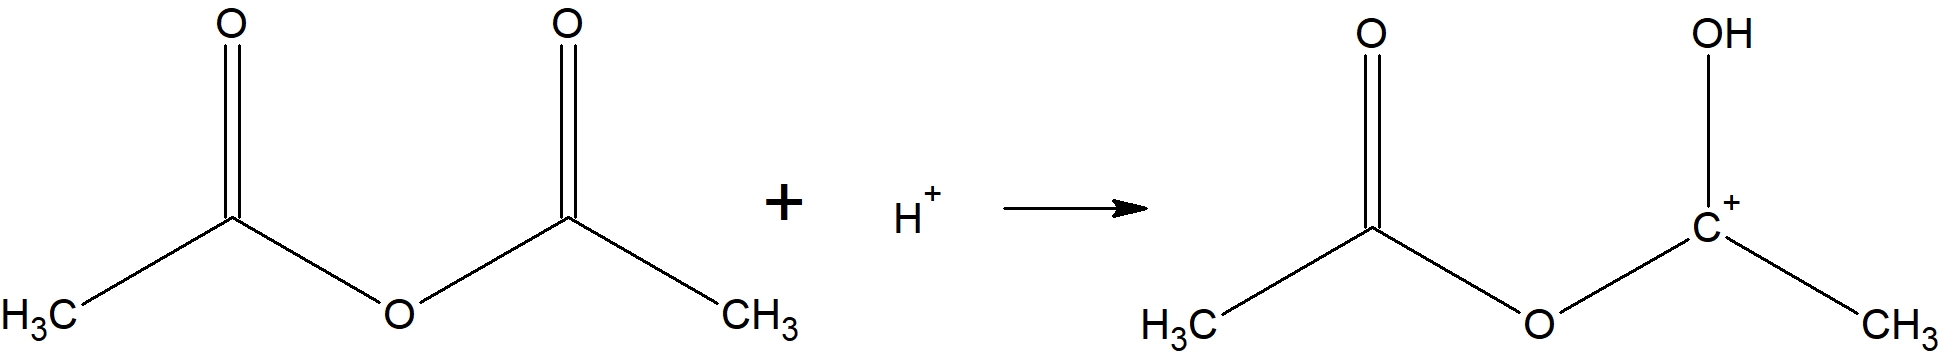
\includegraphics[width=0.5\textwidth]{img/mechanismus1}
\end{flalign}
\begin{flalign}
	\label{fig:}
	\centering
	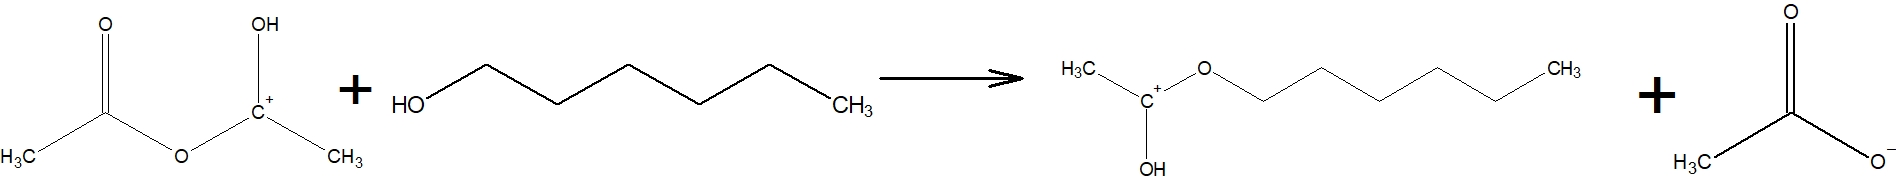
\includegraphics[width=0.9\textwidth]{img/mechanismus2}
\end{flalign}
\begin{flalign}
	\label{fig:}
	\centering
	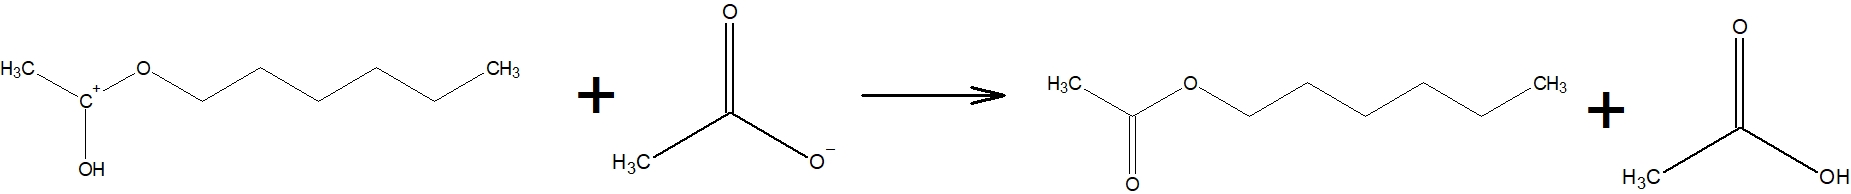
\includegraphics[width=0.9\textwidth]{img/mechanismus3}
\end{flalign}


